\documentclass[11pt]{article}
\usepackage[margin =1in]{geometry}
\usepackage{authblk}
\usepackage{lipsum}
\usepackage{multicol}
\usepackage{graphicx}
\usepackage{float}
\usepackage[hidelinks]{hyperref}
\usepackage{amsmath}
\usepackage[backend = bibtex, style = numeric, sorting = ynt]{biblatex}
\addbibresource{reference.bib}
\title{{\bf Computational Methods for RNA Secondary Structure Prediction}}
\author[1]{Harrison LaBollita}
\author[2]{Petr \u Sulc}
\date{}
\affil[1]{Department of Physics, Arizona State University, Tempe, AZ 85281 USA}
\affil[2]{Center for Biological Physics, Arizona State University, Tempe, AZ 85281 USA}

\begin{document}
\maketitle
\begin{abstract}
\lipsum[1]
\end{abstract}
\tableofcontents
\section{Introduction}
Machine learning exploratory work goes here.

In this report, we  provide an implementation of the Gillespie algorithmn used to model the kinetic folding of RNA secondary structures. We have followed the work \cite{10.1093/nar/gkv480, Kimchi338921} to realize this implementation presented below. However, in this work we introduce a slight modification. Rather than working on the base-pair level, we work at the stem level calculating the reation rate of a stem to form, then create that stem or break depending on where we are at in the algorithmn. We have choosen to work at the stem level for computational speed purposes. We desire to combine multiple computational tools together for predicting the structure of sequences much longer than 100 nucleotides. Therefore, for our alogrithmns to be feasible we must work at the stem level.

It is extremely advantageous to combine both the Gillespie algorithm with the work of Kimichi et. al., because their work accounts for pseudoknot secondary structures, which we know (CITE) many physical RNA structures contain pseudoknots. Thus, making it vital that our algorithms do note make the canoncial (Nussinov, etc.) approximation that the structure does not contain pseudoknot stems.
\section{Convolutional Neural Network Predicts Secondary Structure}
\subsection{Data and Methods}
\begin{figure}[H]
\centering
\hspace*{-8cm}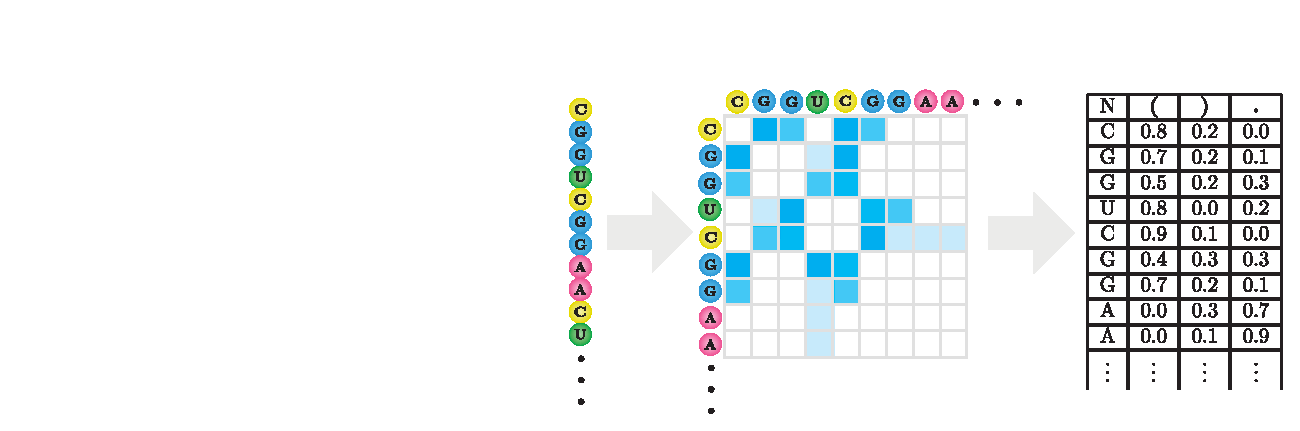
\includegraphics{fig/cnn_model_outline}
\end{figure}
\lipsum[2]
\subsection{Convolutional Neural Network Model}
\lipsum[2]
\subsection{Results}
\lipsum[2]
\section{Stem Level Gillespie Algorithm}
\subsection{Introduction to Gillespie Algorithm}
In \cite{10.1093/nar/gkv480}, the following alogrithm is presented:
\begin{enumerate}
\item Extract the total flux $\Phi$ from the partial sum table.
\item Choose two random numbers $r_{1}$ and $r_{2}$ on the interval $[0, 1]$.
\item  Increment the time by $\tau = - \ln(r_{2})/\Phi$.
\item Identify the first *stem* which satisfies the inequality $$ \sum_{\ell =1} \phi_{\ell} \geq r_{1} \Phi$$ by using our table of reaction rates for each stem. We then recalculate the remainder $\Phi = r_{1} \Phi - \sum_{\ell = 1} \phi_{\ell}$ on the fly.
\item Once this condition is met we choose this stem to form. We make sure it is compatible with all of the other stems in the current structure. If it is not compatible with the current structure, we remove the incompatible pieces and add our new stem. However, if adding this move requires breaking almost all of the current stems then we do not allow this move to occur.
\item Go to Step 1 until the the arbitraty cutoff time has been reached.
\end{enumerate}

\subsection{Stem Level Implementation}

\begin{figure}[H]
\centering
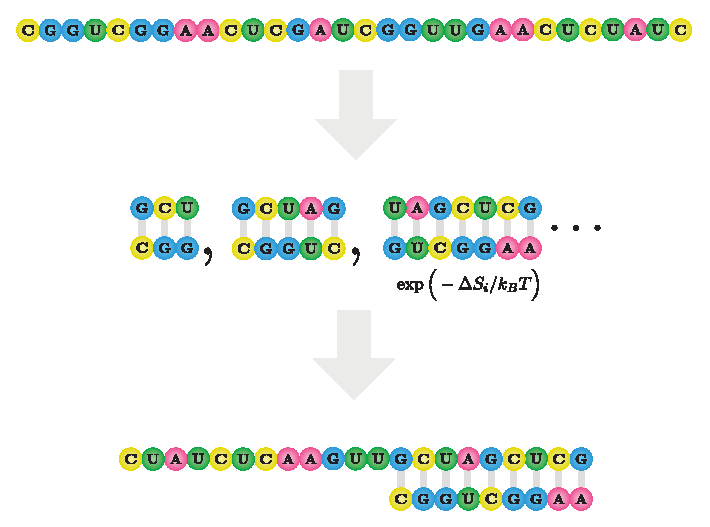
\includegraphics{fig/rna_gillespie_algo}
\end{figure}
\lipsum[2]
\subsection{Results}
\lipsum[2]
\section{Conclusion and Outlook}
\lipsum[2-4]
\lipsum[2-4]
\newpage
\nocite{*}
\printbibliography
\end{document}
